\graphicspath{{figures/Design/IPController/}}
\chapter{Design of the Inverted Pendulum Controller}\label{sec:IPController}
\todo[inline,author=Jacob]{Start with a blockdiagram that has the actual transfer functions.}

The goal of the controller is to balance the stick in an upright position. The system is seen as a block diagram on \autoref{BlockSystemNoControl}. Which gives the transfer function seen in \autoref{eq:CombModel}
\begin{figure}[htbp]
\centering
\missingfigure{}
\caption{Block diagram of the system the controller will attempt to stabilize.}
\label{fig:BlockSystemNoControl}
\end{figure}

The system is inherently unstable as is evident by the pole in the right half plane of the pole-zero plot as seen on \autoref{fig:pzip}.

\begin{figure}[htbp]
\centering
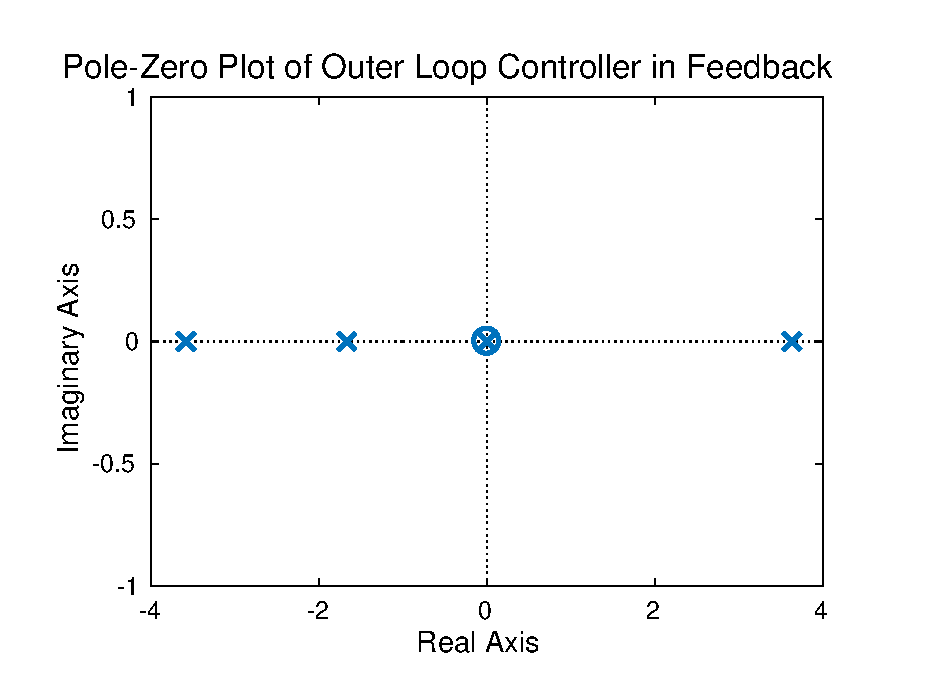
\includegraphics[width=0.6\textwidth]{pzip}
\caption{Pole-zero plot for the inverted pendulums transfer function.}
\label{fig:pzip}
\end{figure}
\todo[inline,author=Jacob]{Check constants found by test and transfer function at the end.}

The problem with the system is the unstable pole in the right half plane and the zeros in 0.

There's a plethora of different options for the controller to use; the simplest being a proportional controller. A simple way to check whether the proportional controller is feasible is by examining the root locus of the transfer function in \autoref{fig:locusIP}. The pole in the right half plane moving towards infinity is caused by the transfer function being negative and can be fixed with a negative gain as shown on figure \autoref{fig:locusNegative}.

\begin{figure}[htbp]
\centering
	\begin{subfigure}{0.45\textwidth}
	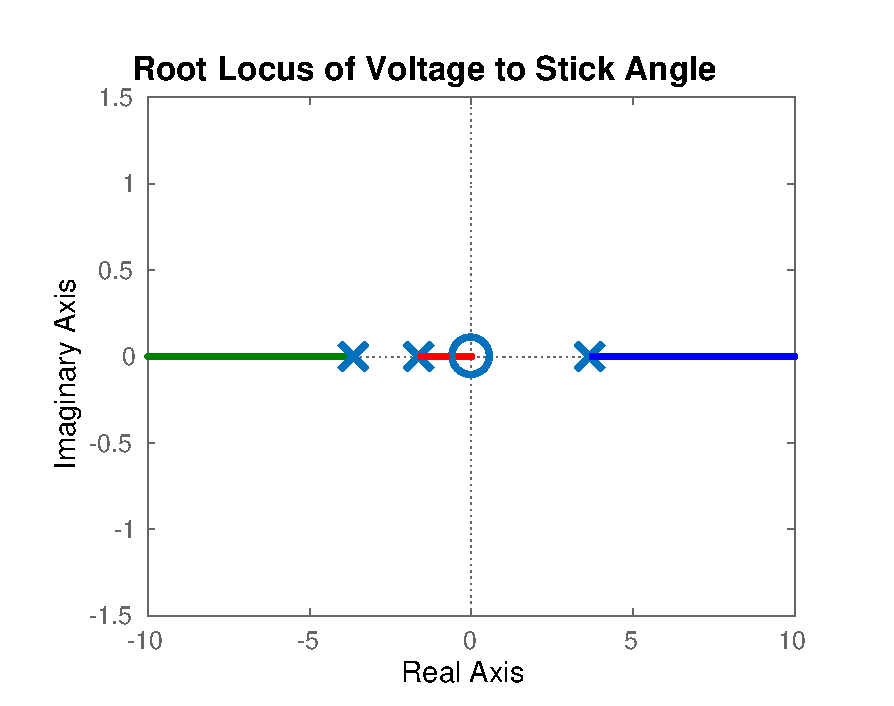
\includegraphics[width=\textwidth]{rlocusplus}
	\caption{Positive gain.}
	\label{fig:locusIP}
	\end{subfigure}
	\begin{subfigure}{0.45\textwidth}
	\centering
	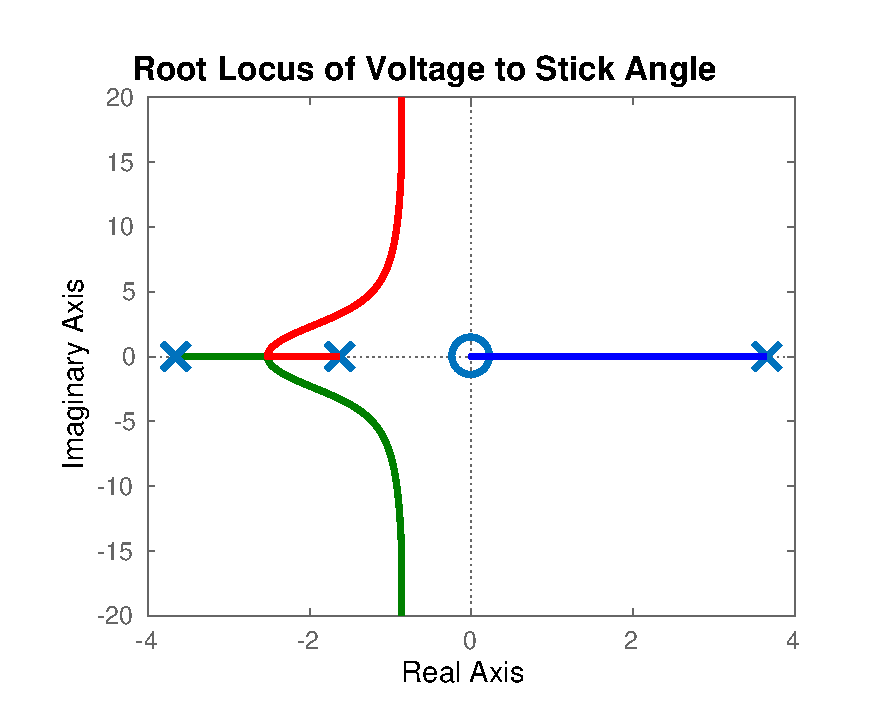
\includegraphics[width=\textwidth]{rlocusminus}
	\caption{Negative gain.}
	\label{fig:locusNegative}
	\end{subfigure}
\caption{Root locus of the inverted pendulums transfer function.}
\end{figure}

The proportional controller isn't feasible as the pole in the right half plane never enters the stable region even with a negative gain. This is because the pole will always end at a zero if available. The zero in 0 blocks the unstable pole from moving into the stable region.

The controller can be simplified by using cascade control. This means two controllers should be designed; one that controls the angle of the arm and one that controls the angle of the stick. The cascade control system can be seen on \autoref{fig:IPCascade}.

\begin{figure}[htbp]
\centering
\includegraphics[width=\textwidth]{IPCascade}
\caption{Block diagram of the inverted pendulum system with cascade control.}
\label{fig:IPCascade}
\end{figure}

If the inner loop is fast enough compared to the outer loop, it is negligible to the outer loop controller. This means the root locus of the can be split into two separate systems with a respective controller that needs to be designed. These two new loops which will be now referred as respectively inner loop and outer loop have their transfer function define in \autoref{eq:InnerOuterTF}.

\begin{subequations}\label{eq:InnerOuterTF}
	\begin{flalign}
		\frac{\Theta_a}{U}&=\\
		\frac{\Theta_s}{\Theta_a}&=
	\end{flalign}
\end{subequations}

The root locus of the two subsystems is seen on \autoref{fig:locusSplit}.
\begin{figure}[htbp]
\centering
	\begin{subfigure}{0.45\textwidth}
	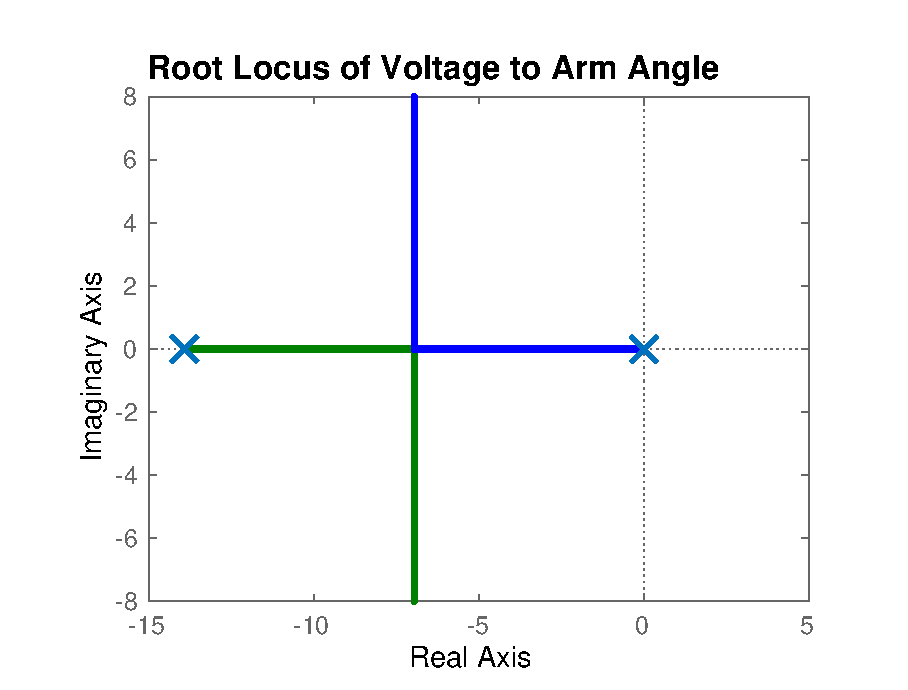
\includegraphics[width=\textwidth]{rlocusVArmAlt}
	\caption{Voltage as input and angle of the arm as output.}
	\label{fig:locusVArm}
	\end{subfigure}
	\begin{subfigure}{0.45\textwidth}
	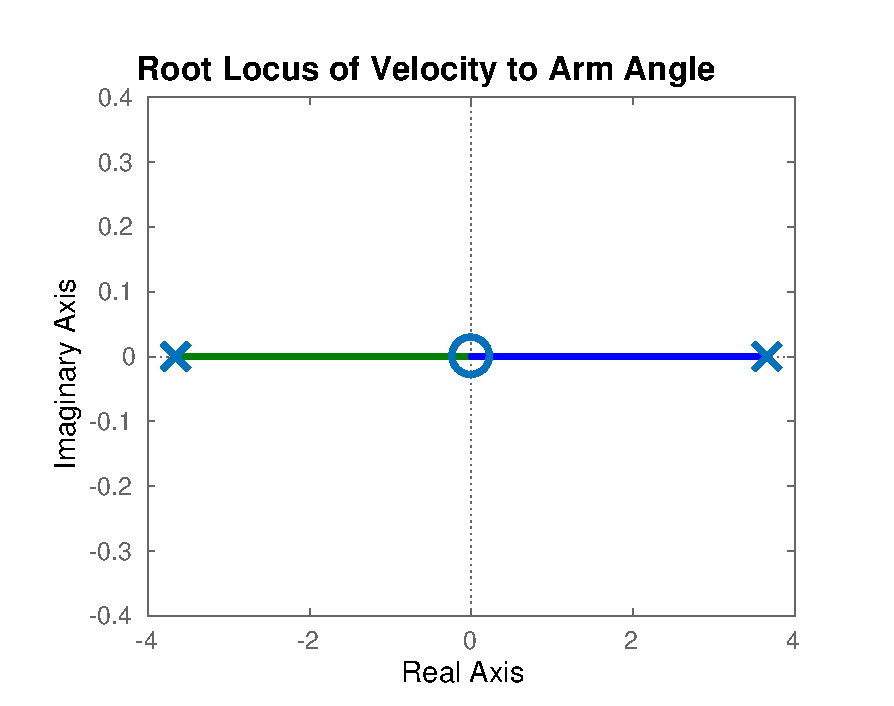
\includegraphics[width=\textwidth]{rlocusArmStick}
	\caption{Angle of the arm as input and angle of the stick as output.}
	\end{subfigure}
\caption{Root locus of the inner loop and outer loop.}
\label{fig:locusSplit}
\end{figure}

With this split it's simpler to design a controller that can move the unstable pole to the stable region. The inner loop controller will be designed first as it's essential to this split that the inner loop is faster than the outer loop. The inner loop controller will be designed to be as fast as possible before the outer loop controller is designed.

\section{Design of Inner Loop Controller}

For the design of the inner loop controller it's important that it settles faster than the outer loop controller without any overshoot. This means the natural frequency of the system with the controller needs to be larger and the poles close to the real axis. The root locus for the motor to the arm on \autoref{fig:locusVArm} shows that a simple gain can not increase the natural frequency without have any overshoot. As such a P controller is chosen as it will increase the rise time and the settling time. With the help of \autoref{fig:VArmGeneralPControllerRLocus} a gain of 9.17 is chosen as it is the maximum gain obtainable without having any overshoot.

\begin{figure} [htbp] 
	\centering
	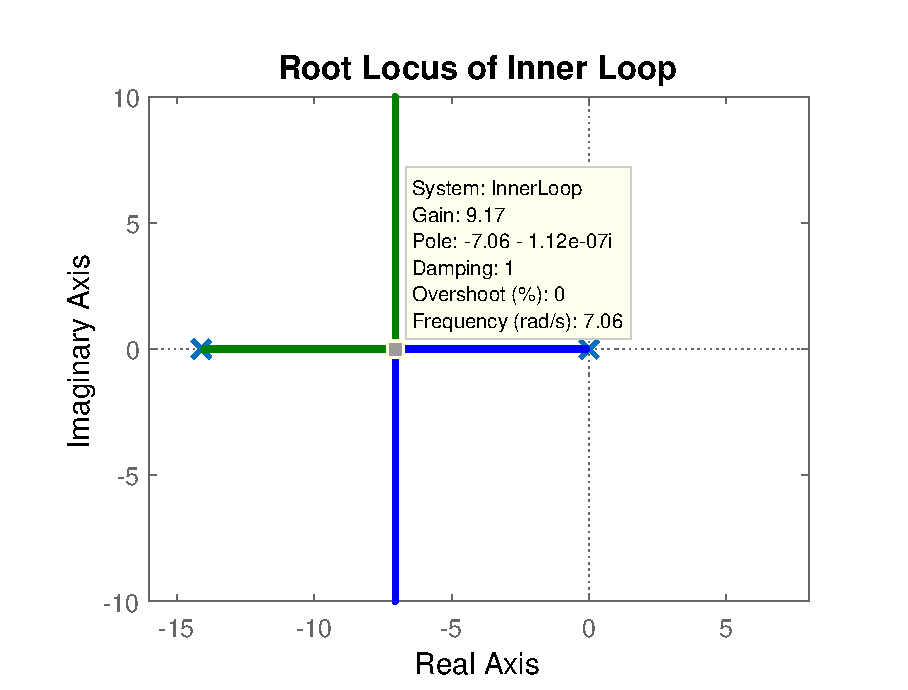
\includegraphics[width=0.7\textwidth]{rlocusVArmGeneralPController.eps}
	\caption{Voltage as input and Arm's angle as the output}
	\label{fig:VArmGeneralPControllerRLocus}
\end{figure}

However this system has only a natural frequency of \SI{6.97}{\radian\per\second} meaning the arm should be quite slow with this controller. This supposition is confirmed by the step response seen in \autoref{fig:VArmGeneralPControllerStepResp}.

\begin{figure} [htbp] 
	\centering
	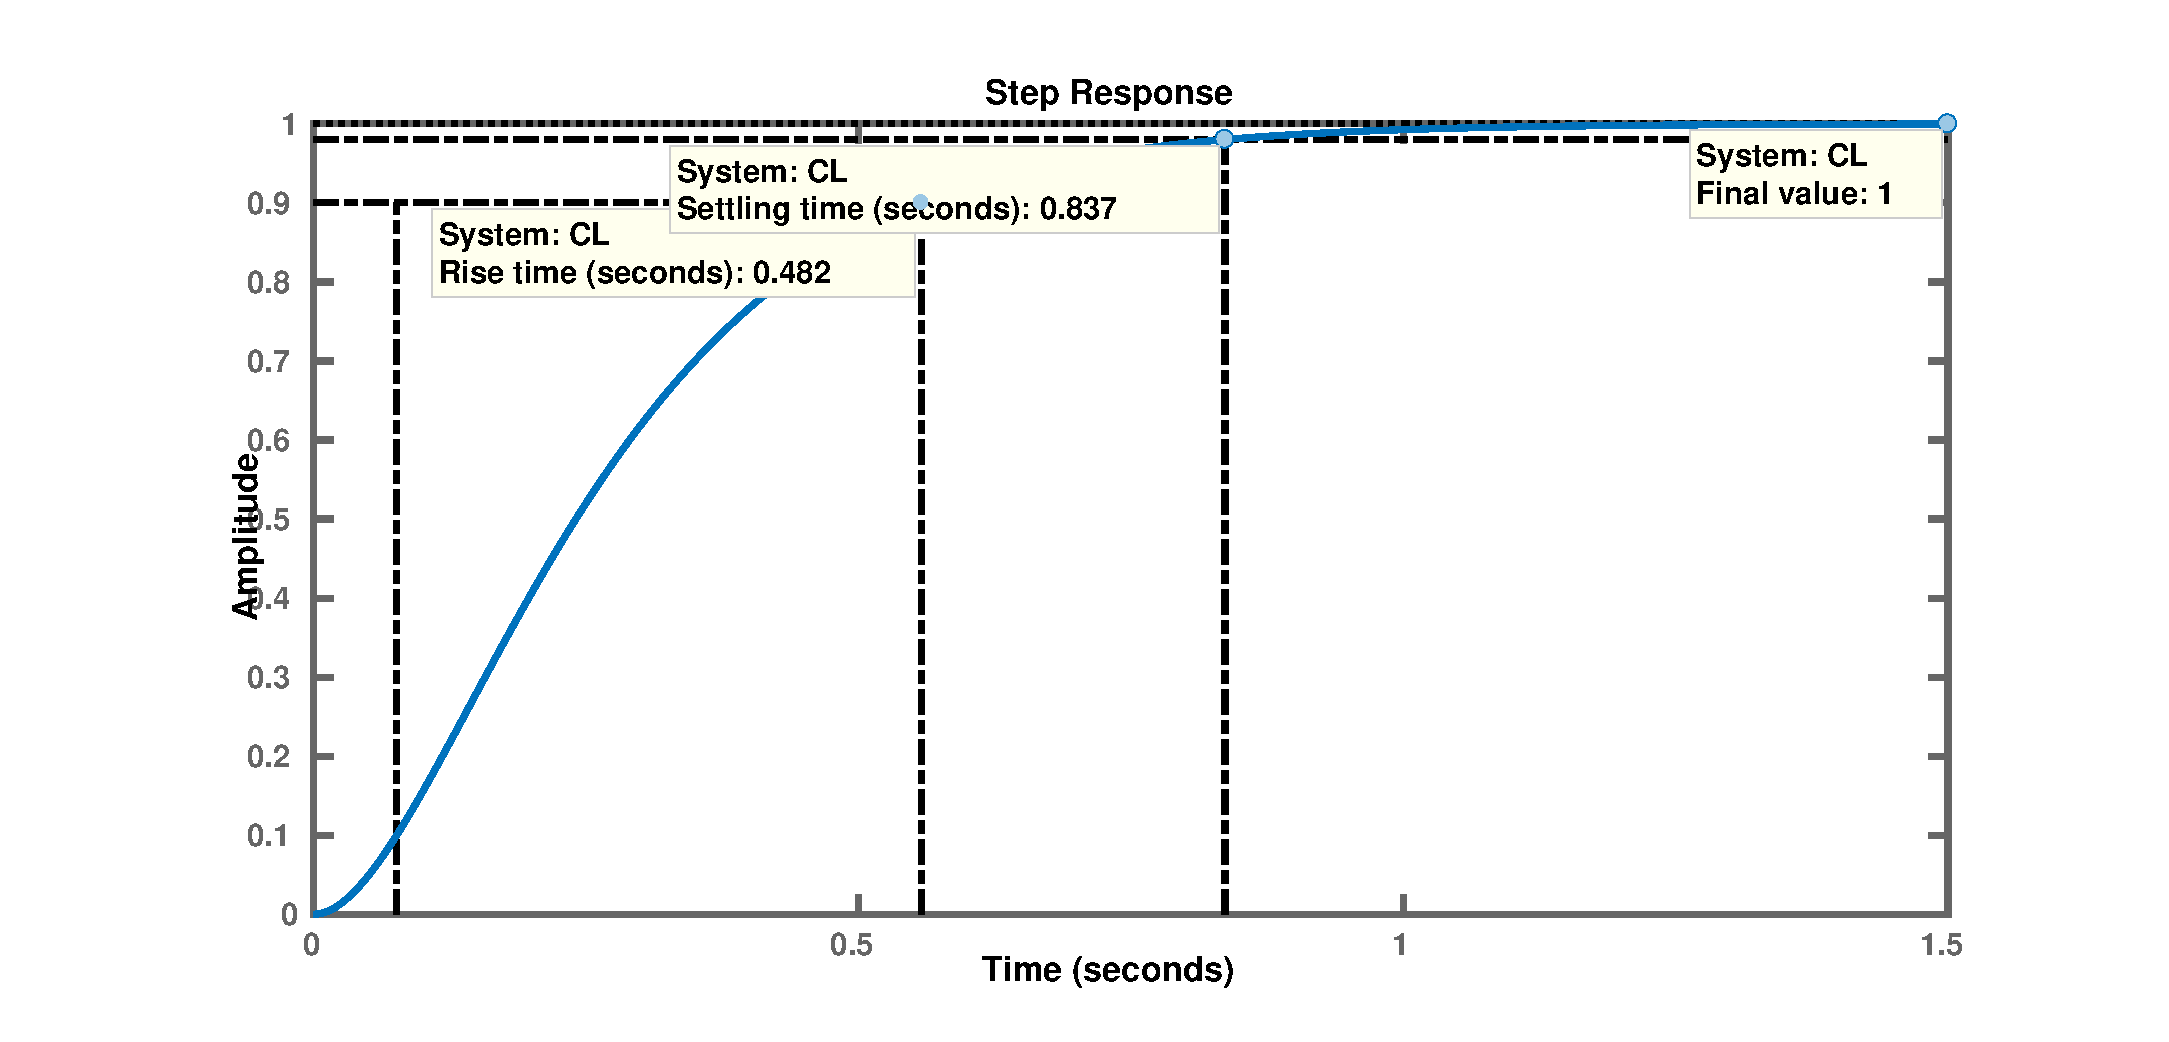
\includegraphics[width=0.8\textwidth]{rlocusVArmGeneralPControllerStepResp.eps}
	\caption{Step response of the arm with the voltage as the input}
	\label{fig:VArmGeneralPControllerStepResp}
\end{figure}
\todo[inline,author=maxime]{add the characteristics of the step response as my computer can't do it for some reasons}

In order to speed up the inner loop two options are available. The first one is to use more elaborate controller than the P controller such as a PD controller or a lead. The second one is to once again divide the inner loop into two loops. The second method is chosen for two reasons. The first one is that since the motor has already a tachometer integrated, and so it is simpler to implement this method. The other one was a problem noticed during the test of the motor for its modeling. The driver is not delivering a constant speed for a constant voltage. And so a feedback loop of the velocity would be able to reduce the inconsistencies generated by the driver. The two new loops are respectively the voltage as the input and the velocity which will be called motor loop from now on, and the velocity as the input and the arm's angle as the output named as arm's loop.

The first loop wich will be designed will be the motor loop as it is the most inner loop.

%\subsection{Design of the Motor Loop Controller}\label{sec:MotorLoop}

The very first loop control is the one adjusting the motor velocity, $\omega_m$, according to the voltage. The loop is seen as a block diagram on \autoref{fig:BlockMotorLoop}.

\begin{figure} [htbp]
	%\hspace*{-3.5cm}
	\centering
	\includegraphics[width=\textwidth]{figures/FigureIsComing}
	\caption{Block diagram of the input/output of the motor loop.}
\end{figure}

The transfer function from $U_m$ to $\omega_{m}$ is taken from \autoref{sec:ModelDCMotor}. \autoref{eq:DCModelNoL} is used with the values for each of its variables: 
\begin{flalign}
\frac{\Omega_m(s)}{U_m(s)}=\frac{0.0293}{3.633\text{e}^{-5}s+0.03138} 
\end{flalign} 

The transfer function has a negative pole making the system stable. A P-controller is enough to control this loop. As it is the most inner loop of the system, the step response has to be faster than the outer loops controlling the arm and the stick. The root locus of the motor loop is plotted next to its step response. 

\begin{figure}[htbp]
	\centering
	\begin{subfigure}{0.48\textwidth}
		\includegraphics[width=\textwidth]{figures/Design/MotorLoop/MotorRootLocus}
		\caption{Root locus of the motor transfer function}
		\label{fig:MotorRootLocus}
	\end{subfigure}
	\begin{subfigure}{0.5\textwidth}
		\centering
		\includegraphics[width=\textwidth]{figures/Design/MotorLoop/MotorStepUncontrolled}
		\caption{Step response of the uncontrolled close loop transfer function}
		\label{fig:fig:MotorStepUncontrolled}
	\end{subfigure}
	\caption{Root locus and step response of the motor loop}
\end{figure}

\autoref{fig:MotorRootLocus} confirms that the motor loop is naturally stable. However, there is a steady state error. The system is then controlled by a P-controller with a gain of 10. 
\begin{figure} [htbp]
	%\hspace*{-3.5cm}
	\centering
	\includegraphics[width=0.8\textwidth]{figures/Design/MotorLoop/MotorStepControlled}
	\caption{Step response of the controlled motor loop.}
	\label{fig:MotorStepControlled}
\end{figure}

As seen on \autoref{fig:MotorStepControlled}, the controlled loop has a rise time of $2.7\text{e}^{-4}$ seconds, ten times faster than the uncontrolled loop. Moreover, the steady state error has decreased from 7\% to 0.01\%. With a proportional gain of 10, the pole is moved far in the left half plane making the motor loop fast enough to be considered as a wire for the arm.



Now the arm's loop will be designed. The motor loop part has a settling time of \SI{0.0159}{\second}, so the settling time of the arm's loop has to be at least \SI{0.159}{\second} in order to make the assumption that the motor's loop transfer function is equal to 1 for the arm's loop. The new transfer function derived from this approximation is \autoref{eq:WArmLoop}.

\begin{equation}\label{eq:WArmLoop}
	\frac{\Theta_a}{\Omega_m}=\frac{N^3}{s}
\end{equation}

The root locus of \autoref{eq:WArmLoop}, in \autoref{fig:WArmLoopRLocus}, shows that there is theoretically no gain limitation for the arm as the pole moves to the left side plan making the system stable, as long as the gain is high enough. The pole is also always on the real axis which means there will be no overshoot no matter the gain.

\begin{figure} [htbp] 
	\centering
	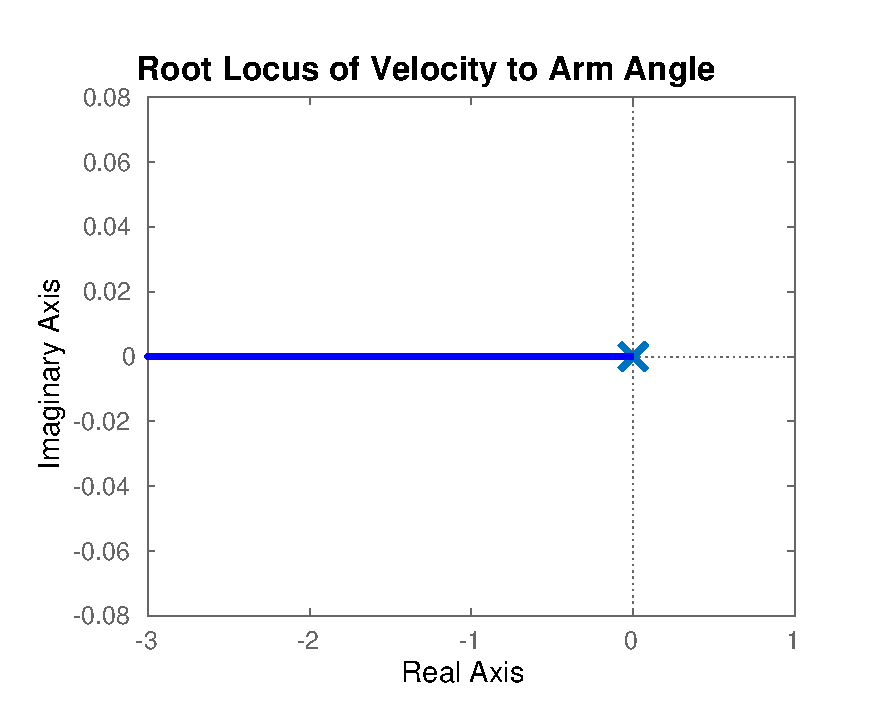
\includegraphics[width=0.7\textwidth]{WArmPControllerRLocus.eps}
	\caption{Velocity as input and Arm's angle as the output}
	\label{fig:WArmLoopRLocus}
\end{figure}

Since it is so our only limitation is the settling time of the motor as explained earlier. A gain of 905 is good enough as it gives a settling time of \SI{0.16}{\second} as seen in \autoref{fig:WArmLoopStepResp}.

\begin{figure} [htbp] 
	\centering
	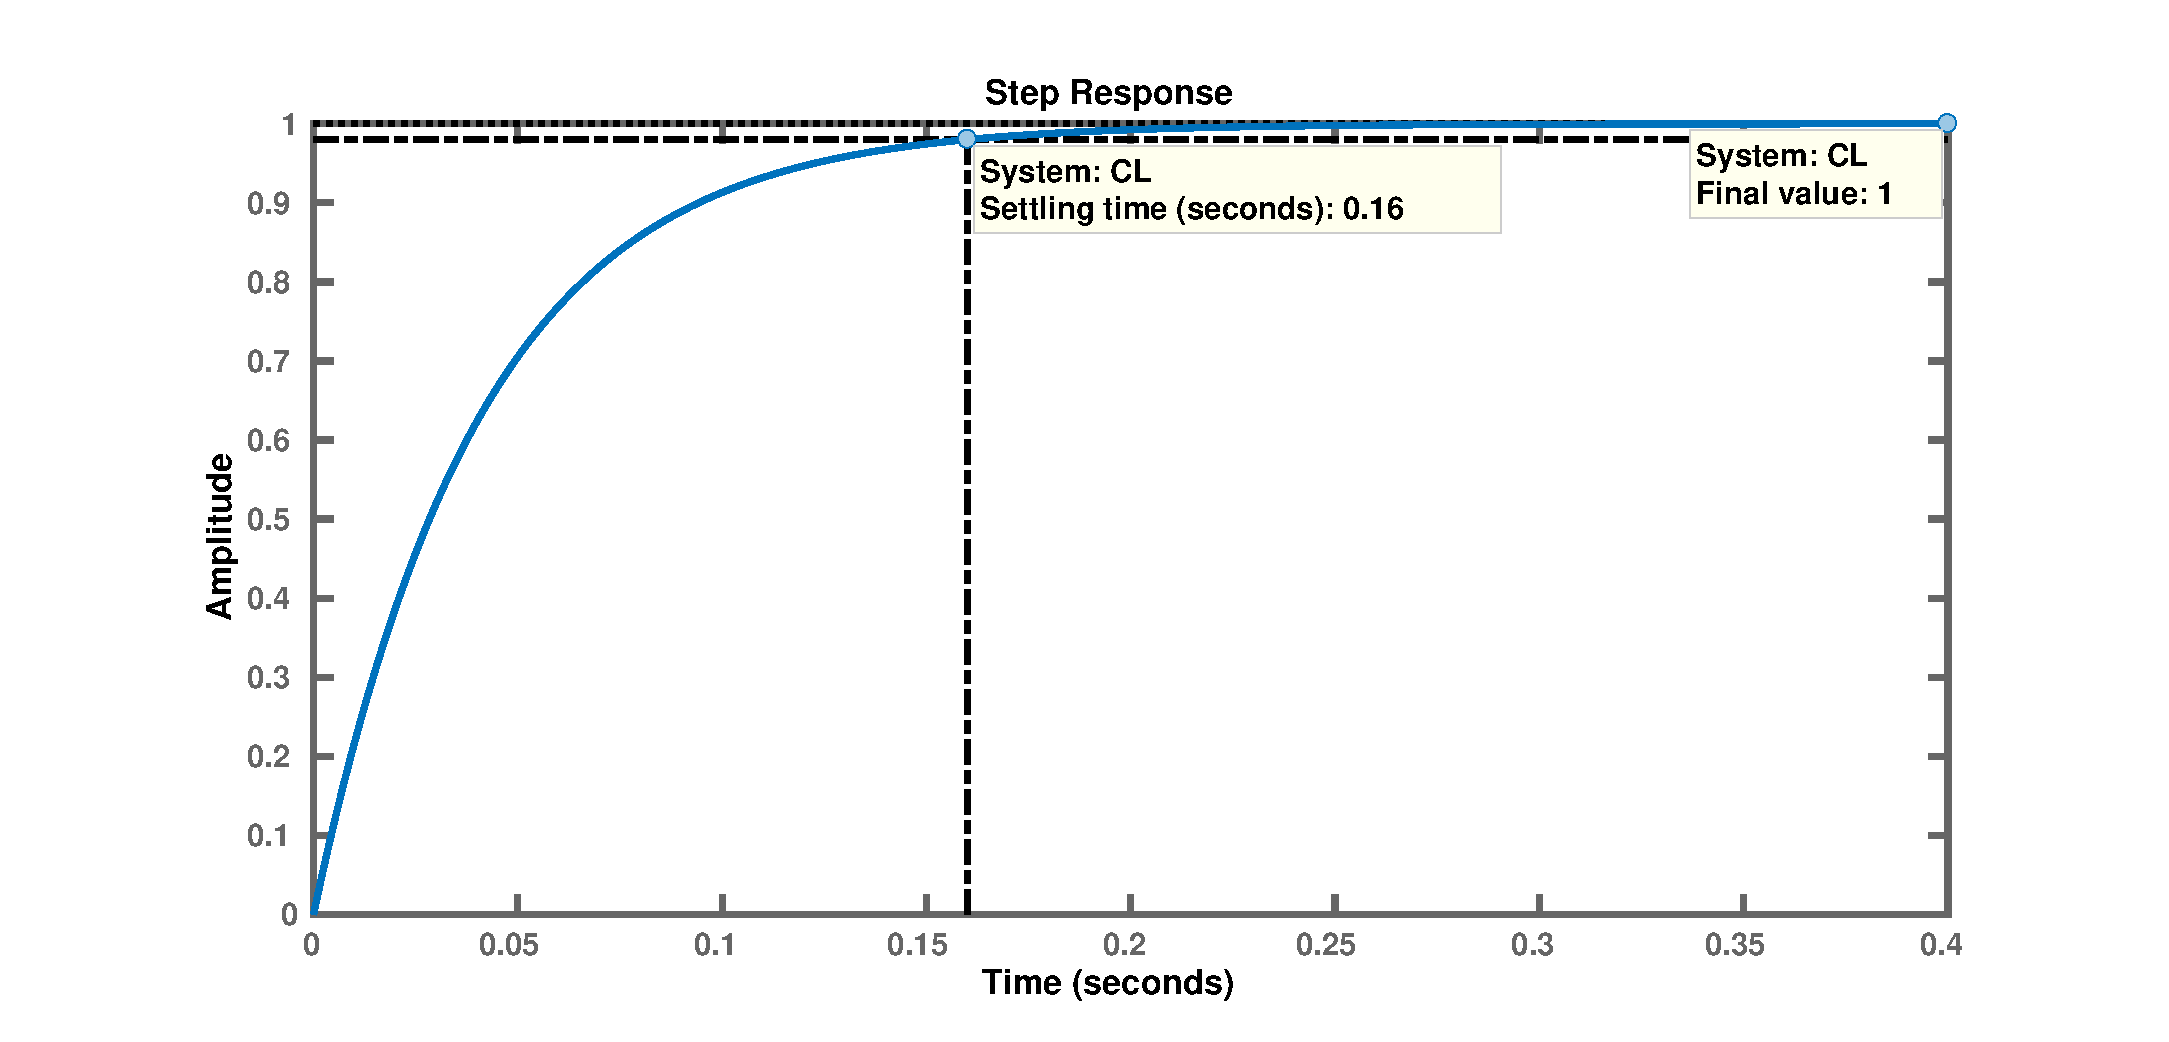
\includegraphics[width=0.8\textwidth]{WArmPControllerStepResp.eps}
	\caption{Step response of the arm's loop}
	\label{fig:WArmLoopStepResp}
\end{figure}

%By moving the zero further into the left half plane gives a faster settling time but requires a higher gain and a faster sampling rate for a digital controller. Having a higher gain can give issues with saturating the motor and there may be limits from the sampling rate with very fast settling times. 

\todo[inline,author=Jacob]{Maybe look into PID as it adds two zeros and is a well documented type of controller. Especially because lead control gives steady state error and the integration can remove it. SSE is terrible for the inner loop but ok for the outer as it's the position and not the angle.}


\section{Design of Outer Loop Controller}
As the poles in feedback will eventually end up at the zeros with a large enough gain, there are two options to bring the unstable pole into the stable region: Remove all zeros in 0 so the pole can cross the into the stable region along the real axis or add another unstable open loop pole to force the poles off the real axis and then try to circumvent the zeros in 0. 

Removing the zeros in 0 can't be done by adding poles as $\inf\cdot0$ isn't defined. Instead it's better to try and redefine the model output to something with a DC gain but at the same time requires the stick to be balanced to achieve the new output. This could be by attempting to control the position of a point on the stick. The stick would need to be balanced in order to have the point always be in the correct position.

%Cancelling zeros in 0 by adding poles can be dangerous as the steady state error will no longer be zero which is critical for a stable inverted pendulum. The system is difficult to control as the transfer function was derived with an attempt to control the angle of the stick. This is only really possible in the special case where the reference is exactly 0 at all times. The system can instead be redefined as trying to control the position of a point on the stick in relation to the vertical axis. By controlling the position instead of the angle would mean the system would still have to balance the stick but not be forced to use a reference of 0 at all times. This could make the system easier to control.

\subsection{Redefining the Inverted Pendulums Output}
The inverted pendulum model will be redefined so the output is the distance from a point on the stick to the vertical axis instead of the angle of the stick. The point, $\alpha$, and the distance to the vertical axis, $x_\alpha$, are seen on \autoref{fig:modelDist}.

\begin{figure}[htbp]
\centering
\includegraphics[width=0.7\textwidth]{ModelDist}
\caption{Diagram of the distance that will be controlled instead of the angle of the stick.}
\label{fig:modelDist}
\end{figure}

The distance to the point can be described by \autoref{eq:xa}.
\begin{flalign}\label{eq:xa}
& x_\alpha(t) = l_a\sin(\theta_a(t))+l_\alpha\sin(\theta_s(t))
\end{flalign}
This is not a linear equation and needs to be linearized in order to Laplace transform it. This is done with a 1st order Taylor approximation around the equilibrium where $\theta_a=\theta_s=0$ in \autoref{eq:xaTaylor}
\begin{subequations}\label{eq:xaTaylor}
\begin{flalign}
& x_\alpha(t)\approx l_a\sin(0)+l_a\cos(0)\theta_a(t)+l_\alpha\sin(0)+l_\alpha\cos(0)\theta_s(t) \\
& x_\alpha(t)\approx l_a\theta_a(t)+l_\alpha\theta_s(t)
\end{flalign}
\end{subequations}
This will then be Laplace transformed in \autoref{eq:xaLaplace}.
\begin{flalign}\label{eq:xaLaplace}
X_\alpha(s)=l_a\Theta_a(s)+l_\alpha\Theta_s(s) 
\end{flalign}

By isolating $\Theta_s(s)$ in \autoref{eq:tfArmStick} and inserting it into \autoref{eq:xaLaplace}, the transfer function in \eqref{eq:xatf} is found. The friction part is removed per \autoref{tab:IPModelVar}.

\begin{subequations}
\begin{flalign}
& X_\alpha(s)=l_a\Theta_a(s)+l_\alpha\frac{-\frac{3l_a}{2l_s}s^2}{s^2-\frac{3g}{2l_s}}\Theta_a(s) \\
& X_\alpha(s)=\frac{l_a\left(s^2-\frac{3g}{2l_s}\right)+l_\alpha\left(-\frac{3l_a}{2l_s}s^2\right)}{s^2-\frac{3g}{2l_s}}\Theta_a(s) \\
& \frac{X_\alpha(s)}{\Theta_a(s)} = \frac{s^2\left(l_a-l_\alpha\frac{3l_a}{2l_s}\right)-l_a\frac{3g}{2l_s}}{s^2-\frac{3g}{2l_s}} \label{eq:xatf}
\end{flalign}
\end{subequations}
The transfer function still ends up with 2 zeros but it's possible to remove them by selecting the point $\alpha$ so $l_\alpha=\frac{2l_s}{3}$. Inserting this into \autoref{eq:xatf} the transfer function becomes \autoref{eq:xaTF}.
\begin{flalign}\label{eq:xaTF}
& \frac{X_\alpha(s)}{\Theta_a(s)} = \frac{-l_a\frac{3g}{2l_s}}{s^2-\frac{3g}{2l_s}}
\end{flalign}

The zeros in 0 has been removed but the distance, $x_\alpha$, now needs to be measured for the feedback. This can be done by measuring the angles, which was also necessary before, but now use \autoref{eq:xa} to calculate the distance instead of using the angle directly. The controller for the transfer function in \autoref{eq:xaTF} can now be designed.
\subsection{Controlling the Distance from the Stick to Vertical}
%The controller for the system will be split into two. One controller in an inner loop that controls the angle of the arm and one in an outer loop that controls the position of the stick. The system with the two controllers can be seen on the block diagram on \autoref{fig:IPBlock}.
%
The new block diagram for the controllers can be seen on \autoref{fig:IPBlock}.
\begin{figure}[htbp]
\centering
\includegraphics[width=\textwidth]{IPBlock}
\caption{Block diagram of the inverted pendulum system with inner and outer loop controllers.}
\label{fig:IPBlock}
\end{figure}
%
%If the inner loop is faster than the outer loop then it can be assumed to be irrelevant when designing the outer loop controller.

With the redefined transfer function the outer loop will control the transfer function in \autoref{eq:xaTF}. From the root locus in \autoref{fig:locusxa} it can be seen that a zero needs to be added on the real axis in the left half plane in order to move the pole in the right half plane to the stable region. 

\begin{figure}[htbp]
\centering
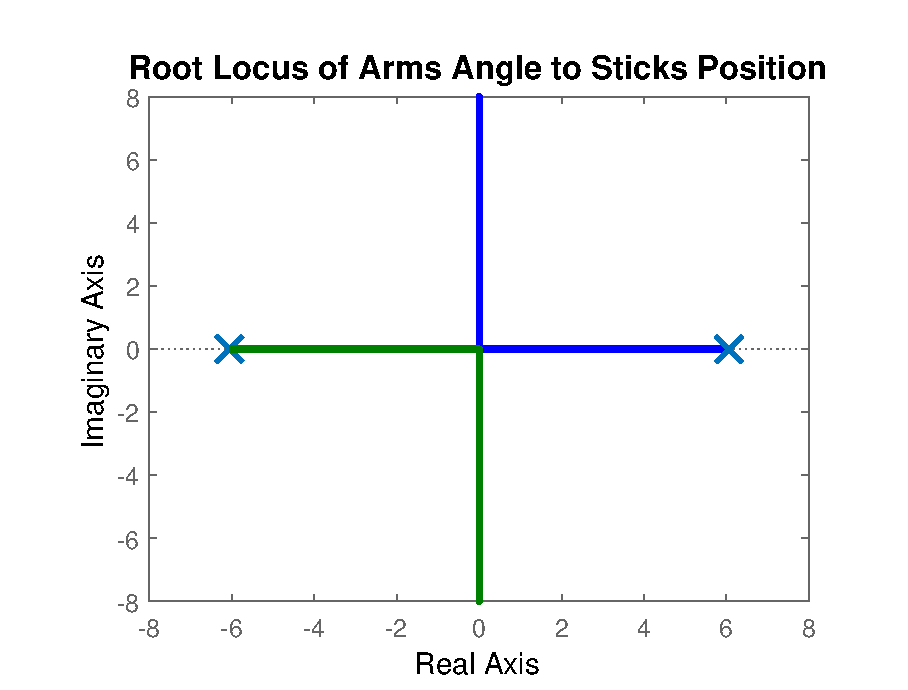
\includegraphics[width=0.7\textwidth]{rlocusRedef}
\caption{Root locus of the transfer function from the angle of the arm to the position of a point on the stick.}
\label{fig:locusxa}
\end{figure}

If the zero is positioned between the two poles both the right most will move towards the zero while the leftmost moves towards infinity; both along the real axis. Positioning the zero close to the origin doesn't allow for the pole to move far into the left half plane. If it's put far to the left of the stable pole the poles will move off the real axis and to the left of the zero with higher gain. This can move them very far into the left half plane before they come back to the real axis which could cause issues for making the inner loop faster than the outer loop. This is because the further away the poles are from origin the higher the natural frequency and a high natural frequency means small settling time. If the poles are off the real axis it'll introduce overshoot which needs to be under 10\% per the specifications. 

Placing the zero close to the leftmost pole would allow for the unstable pole to move further into the left half plane without an overly fast response or any overshoot. 

The zero could theoretically be placed on the pole to cancel it and allow the pole to move further into the left half plane along the real axis. This would be ideal but the true location of the pole of the real system is difficult to find as small variations in measurements of the system could move the pole slightly. 

The zero will initially be placed on the pole as it doesn't change the system drastically whether it's slightly off to either side. The pole is then placed at $-\sqrt{\frac{3g}{2l_s}}$. This can be seen in \autoref{fig:rlocusZeroAdded}.

\begin{figure}[htbp]
\centering
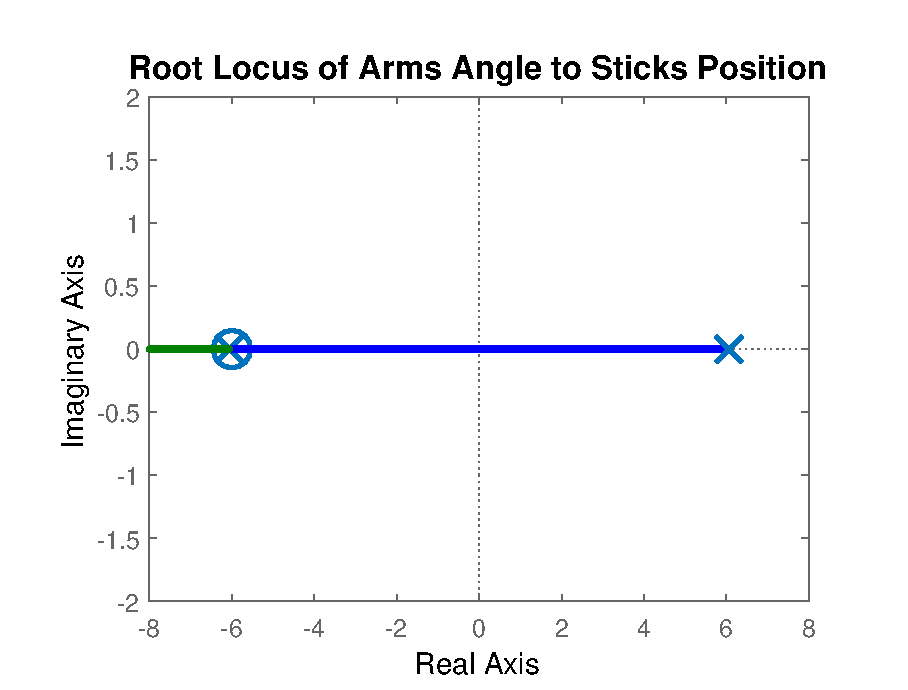
\includegraphics[width=0.7\textwidth]{rlocusZeroAdded}
\caption{Root locus of the outer loop system with a zero cancelling the left pole.}
\label{fig:rlocusZeroAdded}
\end{figure}

The unstable pole can now enter the stable region by selecting a gain large enough. Simply adding a zero to the system will however amplify high frequencies. This can be avoided by adding a pole further into the left half plane. This effectively makes the controller a lead controller. The position of the pole and the gain will determine the settling time and overshoot of the system. The settling time for the outer loop controller should be more than 10 times slower so the assumption, that the inner loop controller is much faster than the outer loop controller, holds true. As the gain increases the two poles move closer to each each other before meeting and moving into the imaginary plane. The gain will be selected to be however much is needed for the poles to meet. The pole can then be selected such that the place where the poles meet will give a settling time 10 times slower than the inner loop.

As the settling time of the inner loop is \textbf{TBD!} the natural frequency of the outer loop needs to be \textbf{TBD/10}. To achieve that the lead controller pole needs to be placed so the halfway point between it and the unstable pole is \textbf{TBD/10}. The pole location then becomes \textbf{MAYBE AN EQUATION?!?}. This can be seen on \autoref{fig:rlocusLead}.
\begin{figure}[htbp]
\centering
\missingfigure{}
\caption{Root locus of the outer loop with the lead controller.}
\label{fig:rlocusLead}
\end{figure}

To make the two poles meet a gain of \textbf{TBDGain} is needed. This gives a lead controller of \autoref{eq:IPLead}.
\begin{flalign}
D_{x}=G\frac{s+\sqrt{\frac{3g}{2l_s}}}{s+p}\label{eq:IPLead}
\end{flalign}

%Selecting the gain too large will however move the other pole further into the left half plane making it more difficult to make the inner loop system faster than the outer loop. As both the zero placement and gain needs to be adjusted later in conjunction with the inner loop controller, the gain will be set to 1 as this puts the unstable pole in the left half plane without the other pole moving too far away as seen on the pole-zero plot on \autoref{fig:pzouterloop}.
%\begin{figure}[htbp]
%\centering
%\includegraphics[width=0.7\textwidth]{pzouterloop}
%\caption{Pole-zero plot of the system with the outer loop controller in feedback.}
%\label{fig:pzouterloop}
%\end{figure}







%\todo[inline,author=Jacob]{For the rest of this section: Use root locus to design Dx controller (Maybe parts of next section can be used here), then design Dm controller while keeping in mind it should be faster than Dx. I'd like for the angle of the stick to somehow be shown as a disturbance in the system and relate the redefinition to feedforward control for better disturbance rejection if possible. Tune parameters in the end as inner loop will have an effect on outer loop.}

%\section{Controller with a 2nd right half plane pole added}
%\todo[author=Jacob, inline]{A lot of this only applies for 2nd order system which this is not. I already wrote it without considering that so this section might have to be deleted but I'm leaving it for now. 2 zeros in 0 is also a massive pain in the ass.}
%A different control method will be attempted in this section where the model won't be redefined but rather a 2nd pole will be added to the right half plane in an attempt to circumvent the zeros in 0.
%
%This controller adds a zero and a pole to the system and thus have three variables that needs to be chosen: The gain and the locations of the zero and the pole. The pole has to be located somewhere in the right half plane and the zero in the left. Their exact locations influence the root locus of the system.
%
%To make the system as stable as possible a fast rise time and low overshoot is desirable. From the specifications the overshoot is set as maximum 10\% with no requirements for the rise time. The damping ratio, $\zeta$, can be found from the overshoot percentage, $M_p$, by \autoref{eq:IPOvershoot}.
%\begin{subequations}
%\begin{flalign}
%& M_p=100\exp^{\frac{-\pi\zeta}{\sqrt{1-\zeta^2}}}<10\%  \\
%& \zeta = \sqrt{\frac{\left(\ln{\frac{M_p}{100}}\right)^2}{\pi^2+\left(\ln{\frac{M_p}{100}}\right)^2}}  \\
%& \zeta > \sqrt{\frac{\left(\ln{\frac{10\%}{100}}\right)^2}{\pi^2+\left(\ln{\frac{10\%}{100}}\right)^2}} = 0.59 \label{eq:IPOvershoot}
%\end{flalign}
%\end{subequations}
%
%The damping ratio then has to be larger than 0.59 in order to have a overshoot of less than 10\% as specified. The rise time, $t_r$, is approximated by \autoref{eq:IPRisetime}.
%\begin{flalign}\label{eq:IPRisetime}
%& t_r =\frac{2.2}{\zeta\omega_n} 
%\end{flalign}
%
%In order to get as fast a rise time as possible the natural frequency and damping ratio both needs to be maximized. The natural frequency can be found on the root locus by the length from the poles to the origin. The damping ratio is found by the angle from the imaginary axis to the poles. As both $\zeta$ and $\omega_n$ are dependent on the pole locations it's possible that the fastest response time comes with a damping ratio below 0.59. The goal of this controller is to minimize \autoref{eq:IPRisetime} but maintaining a damping ratio above 0.59.
%
%The location of the pole, and zero and the gain can thus be decided in order to achieve final pole locations with as far away from the origin as possible while having an angle to the imaginary axis that corresponds to $\zeta=0.59$.

%For the inverted pendulum it's also worth to consider a controller that keeps the arm at zero radians as well as it has a much harder time controlling the arm when out of the upright position. Therefore two controllers will be made: A single-input single-output (SISO) controller that only controls the angle of the stick and a single-input multiple-output (SIMO) controller that controls both the angle of the stick and the arm. 
%\todo[inline,author=Jacob]{If time allows. Otherwise just SISO.}

%\section{Single input single output controller for the inverted pendulum}
%For the SISO controller at least a zero or pole must be introduced along with the P-controller in the system in order to move the pole in the right half plane to the left half plane. For the pole in the right half plane to cross into the left half plane a pole must be added either in 0 to cancel the zero or in the right half plane forcing both off the real axis and allowing them to circumvent the zero in 0 and enter the stable region.

